\documentclass[../../Report.tex]{subfiles}
\usepackage[italian]{babel}

\begin{document}
\chapter{Metodologia}

\section{Data Acquisition}
In uno studio di Data Analysis, lo step di Data Acquisition è il primo della pipeline da seguire.
In questa fase abbiamo raccolto i dati necessari dal dataset \cite[MovieLens]{MovieLens}.
I file sono stati raccolti in una cartella denominata \texttt{ml-25m} contente un README.


\subsection*{Dataset}
\label{dataset}

Movielens è un Recomendation System per contenuti multimediali, quali film, serie tv, documentari ecc.
Movielens mette a disposizione degli sviluppatori un dataset opensource, generator dal database TMDB (The Movie Database).
Questo datasedt contiene recensioni con voti e tag di oltre 60.000 film, raccolte da oltre 150.000 utenti durante il periodo che va dal 1995 fino al 2019.
\\
Il dataset è composto dai seguenti file:
\begin{itemize}
    \item \textit{genome-scores.csv}: contiene il \textit{relevance score} di ogni tag per tutti i film (ovvero, quanto un tag è importante per il dato film).
    \item \textit{genome-tags.csv}: contiene tutti i tag presenti all'interno del dataset.
    \item \textit{links.csv}: contiene gli ID di ogni film per i due database TMBD e IMDB.
    \item \textit{movies.csv}: contiene i titoli dei film, con i rispettivi generi.
    \item \textit{ratings.csv}: contiene più di 25.000.000 votazioni provenienti dalle recensioni degli utenti.
    \item \textit{tags.csv}: contiene i tag che sono stati assegnati ai film dagli utenti nelle rispettivi recensioni.
\end{itemize}

Per il nostro caso di studio, non abbiamo fatto uso di tutti i file disponibili, ma esclusivamente quelli che abbiamo considerato adatti per lo scopo.
Di seguito viene mostrata la struttura dei tali.
\\
Il dataset \textit{\textbf{ratings}} eèstato selezionato per poter far uso dei voti assegnati ai film dagli utenti, per poter quindi ottenere il voto mediio di tali film.
La struttura è la seguente
\begin{table}[H]
    \centering
    \begin{tabular}{|c|c|c|c|}
        \hline
        \textbf{userId} & \textbf{movieId} & \textbf{rating} & \textbf{timestamp} \\
        \hline
        1               & 296              & 5.0             & 1147880044         \\
        1               & 306              & 3.5             & 1147868817         \\
        1               & 307              & 5.0             & 1147868828         \\
        1               & 665              & 5.0             & 1147878820         \\
        1               & 899              & 3.5             & 1147868510         \\
        ...             & ...              & ...             & ...                \\
        \hline
    \end{tabular}
    \caption{ratings.csv}
    \label{tab:ratings_csv}
\end{table}

Il dataset \textit{\textbf{genome-scores}} è stato selezionato per poter identificare le relazioni che ci sono tra un dato voto ed i valori dei tag assegnati
\begin{table}[H]
    \centering
    \begin{tabular}{|c|c|c|}
        \hline
        \textbf{movieId} & \textbf{tagId} & \textbf{relevance}   \\
        \hline
        1                & 1              & 0.028749999999999998 \\
        1                & 2              & 0.023749999999999993 \\
        1                & 3              & 0.0625               \\
        1                & 4              & 0.07574999999999998  \\
        1                & 5              & 0.14075              \\
        ...              & ...            & ...                  \\
        \hline
    \end{tabular}
    \caption{genome-scores.csv}
    \label{tab:genome-scores_csv}
\end{table}



Infine, si è fatto uso del dataset \textit{\textbf{movies}} per ottenere le informazioni inerenti al genere di ogni film.
\begin{table}[H]
    \centering
    \begin{tabular}{|c|c|c|}
        \hline
        \textbf{movieId} & \textbf{title}           & \textbf{genres}              \\
        \hline
        1                & Toy Story (1995)         & Adventur$|$Animation$|$\dots \\
        2                & Jumanji (1995)           & Adventure$|$Children$|$\dots \\
        3                & Grumpier Old Men (1995)  & Comedy$|$Romance             \\
        4                & Waiting to Exhale (1995) & Comedy$|$Drama$|$\dots       \\
        \dots            & \dots                    & \dots                        \\
        \hline
    \end{tabular}
    \caption{movies.csv}
    \label{tab:movies.csv}
\end{table}


\section{Data Visualization}
Nella fase di \textit{data visualization} andremo a visualizzare alcune proprietà e peculiarità del dataset.

\subsubsection{Distribuzione dei ratings}
Nella seguente figura, è mostrata la distribuzione dei voti sul dataset.
\begin{figure}[H]
    \centering
    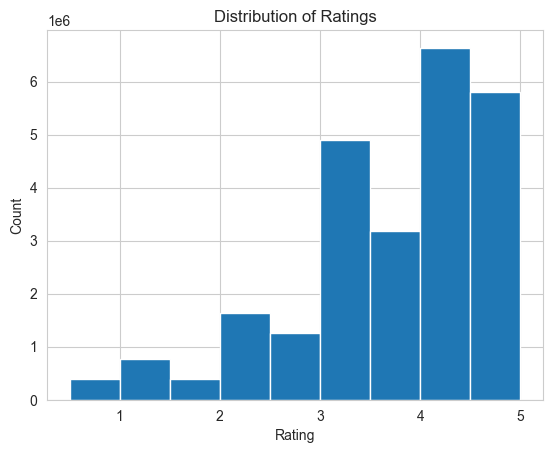
\includegraphics[width = .6\textwidth]{graph_distribution.png}
    \caption{Distribution of Ratings.}
    \label{fig:ratings_distribution_graph}
\end{figure}
Il gafico mostra la distribuzine dei voti sul dataset, evidenziando un chiaro sbilanciamento nella distribuzione. In particolare, si può osservare una concentrzione significativamente maggiore di voti con valore di 3 o superiore rispetto ai voti inferiori.
Questo sbilanciamento è ulteriormente evidenziato dal fatto che i voti con valore di 3 o superiore sono 6 o più volte maggiori rispetto ai voti più bassi.
Tale distribuzione suggerisce una maggiore prevalenza di valutazioni positive rispetto a quelle negative o neutre nel dataset.
Questo risultato potrebbe essere utile per comprendere meglio le caratteristiche del dataset, ad esempio potrebbe suggerire la presenza di una tendenza positiva nelle valutazioni, o la necessità di bilanciare meglio le categorie di voto.
\subsubsection{Relazione tra numero di voti e voto medio}
\begin{figure}[H]
    \centering
    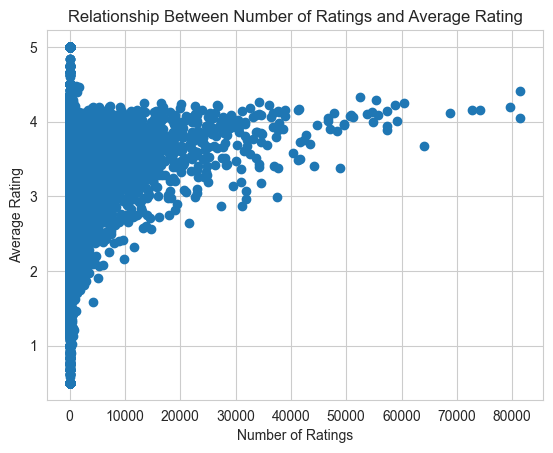
\includegraphics[width = .6\textwidth]{realtionship_between_n_ratings_and_avg.png}
    \caption{Relationship between Number of Ratings and Average Rating.}
    \label{fig:realtionship_between_n_ratings_and_avg}
\end{figure}
Il grafico mostra la relazione tra il numero di voti e il voto medio, evidenziando una tendenza simile ad una funzione esponenziale.
In particolare, il grafico mostra un aumento costante del voto medio all'aumentare del numero di voti, con un picco raggiunto intorno al valore 4.
Tuttavia, a partire da questo punto, si verifica una diminuzione improvvisa del voto medio per poi stabilizzarsi in prossimità del valore neutro.
Questa tendenza suggerisce che il numero di voti ha un impatto significativo sul voto medio ricevuto, in particolare nei casi in cui il numero di voti è relativamente basso.
Tuttavia, per i votio più alti, sembra che la quantità di voti ricevuti non abbia un impatto significativo sul risultato finale. Inoltre, la diminuzione improvvisa del voto medio tra 4 e 5 suggerisce che esiste una soglia critica oltre la quale i voti ricevuti possono avere un effetto negativo sul voto medio complessivo


\subsubsection{Voto medio per Genere}
\begin{figure}[H]
    \centering
    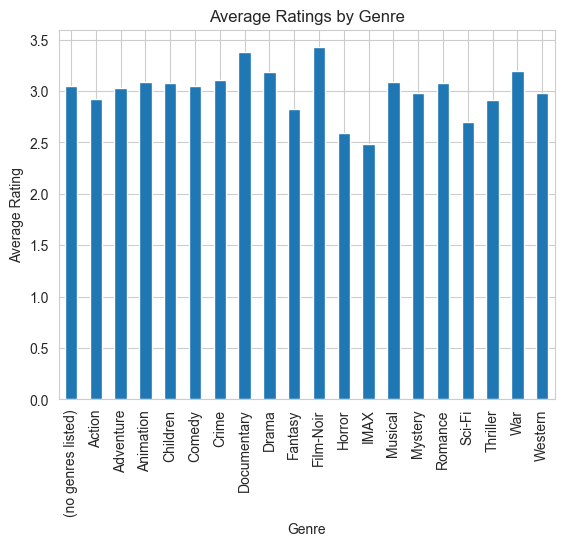
\includegraphics[width = .6\textwidth]{avg_by_genre.png}
    \caption{Average Ratings by Genre.}
    \label{fig:avg_by_genre}
\end{figure}
Il grafico mostra il voto medio per genere e rivela un andamento generalmente stabile, con tutti i valori che si attestano intorno al valore 3.
Alcuni valori si avvicinano al 3.5, indicando una maggiore gradazione positiva, mentre altri si avvicinano al valore 2.5, indicando una maggiore gradazione negativa.
Questa distribuzione dei voti suggerisce che il genere non sembra influenzare significativamente il voto medio complessivo, ma piuttosto, la valutazione sembra essere determinata in base alle caratteristiche specifiche della valutazione stessa.
Tuttavia, esistono alcune differenze tra i voti attribuiti dai generi, con alcune categorie che mostrano una maggiore tendenza verso valutazioni positive rispetto ad altre. 
Ad esempio, il genere "commedia" sembra essere valutato in modo più positivo rispetto al genere "drammatico". 
Questi risultati potrebbero suggerire che le preferenze personali dei valutatori infuenzano le loro valutazioni, oltre alle caratteristiche del film stesso.



\section{Tabular Data}

\end{document}
